%!TEX TS-program = Arara
% arara: pdflatex: {shell: yes}
\documentclass[12pt,ngerman]{scrartcl}

\usepackage[utf8]{inputenc}
\usepackage[T1]{fontenc}
\usepackage{booktabs}
\usepackage{babel}
\usepackage{graphicx}
\usepackage{csquotes}
\usepackage{paralist}
\usepackage{xcolor}
\usepackage[]{tikz}
\usepackage[]{pgfplots}

\begin{document}

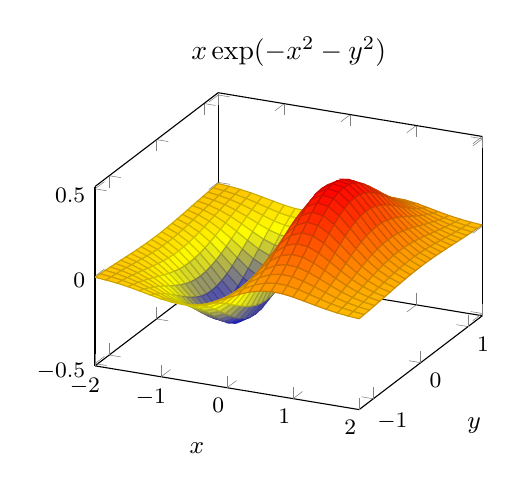
\begin{tikzpicture}
\begin{axis}[
title={$x \exp(-x^2-y^2)$},
xlabel=$x$, ylabel=$y$,
small,
]
\addplot3 [
surf,
domain=-2:2,
domain y=-1.3:1.3,
] {exp(-x^2-y^2)*x};
\end{axis}
\end{tikzpicture}

\end{document}